\section{Risultati ottenuti}
\subsection{Metriche utilizzate per detection su singole immagini}
Nell'ambito della computer vision vengono tipicamente utilizzate due tipi di metriche per misurare due diverse proprietà:
\begin{itemize}
\item Corretta determinazione della posizione degli oggetti;
\item Rilevamento dell'esistenza degli oggetti nell'immagine e la loro corretta classificazione.
\end{itemize}
Le metriche utilizzate per misurare la bontà dei risultati del progetto sono F1, AP (Average Precision) e mAp (mean Average Precision) le quali misurano la seconda proprietà sopra elencata.
Prima di iniziare a descrivere le metriche è necessario definire alcuni concetti che saranno poi coinvolti per il calcolo dei valori delle metriche.
\subsubsection{Precision}
La precision misura l'accuratezza delle classificazioni ed indica la percentuale di classificazioni corrette sulla base di quelle totali e viene calcolata come:
\[
    precision = \frac{TP}{TP + FP}
\]
Dove TP (True Positives) è il numero di classificazioni corrette e FP (False Positives) è il numero di classificazioni errate. E' da sottolineare che se uno stesso elemento viene individuato più di una volta, solo la prima volta conterà come TP mentre il resto delle volte conterà come FP. Questa metrica fornisce un'idea sulla correttezza dei risultati.
\subsubsection{Recall}
La recall misura quanti oggetti sono stati individuati e classificati correttamente sulla base degli oggetti totali, viene calcolata come:
\[
    recall = \frac{TP}{TP + FN}
\]
Dove TP (True Positives) è sempre il numero di classificazioni corrette mentre FN (False Negatives) è il numero di di oggetti che non sono stati individuati ma che se sarebbe stato corretto individuare. Questa metrica fornisce un'idea sulla completezza dei risultati.
\subsubsection{F1}
F1 è una metrica che combina la precision con il recall e può essere interpretata come la media armonica tra la precision e la recall. Il valore massimo ottenibile è 1 raggiungibile nel caso in cui sia la precision che la recall siano pari ad 1 mentre il valore minimo è 0 ottenuto quando entrambe le metriche che lo compongono assumono valore pari a 0. Viene calcolato come:
\[
    F1 = 2 \times \frac{precision \times recall}{precision + recall}
\]
\subsubsection{Intersection over union}
L'intersection over union (IoU) misura il grado di sovrapposizione tra due aree e viene usato per misurare il grado di sovrapposizione tra la box dell'oggetto individuato e la box dell'oggetto reale. Viene calcolata come:
\[
    IoU = \frac{AI}{AU}
\]
Dove AI (Area dell'Intersezione) corrisponde all'area dell'intersezione tra le due bounding boxes e AU (Area dell'Unione) corrisponde all'area dell'unione tra le due bounding boxes.
Una label per essere considerata come corretta deve avere un valore di IoU maggiore di una soglia stabilità (per esempio 0.5).
\begin{figure}[H]
	\centering
	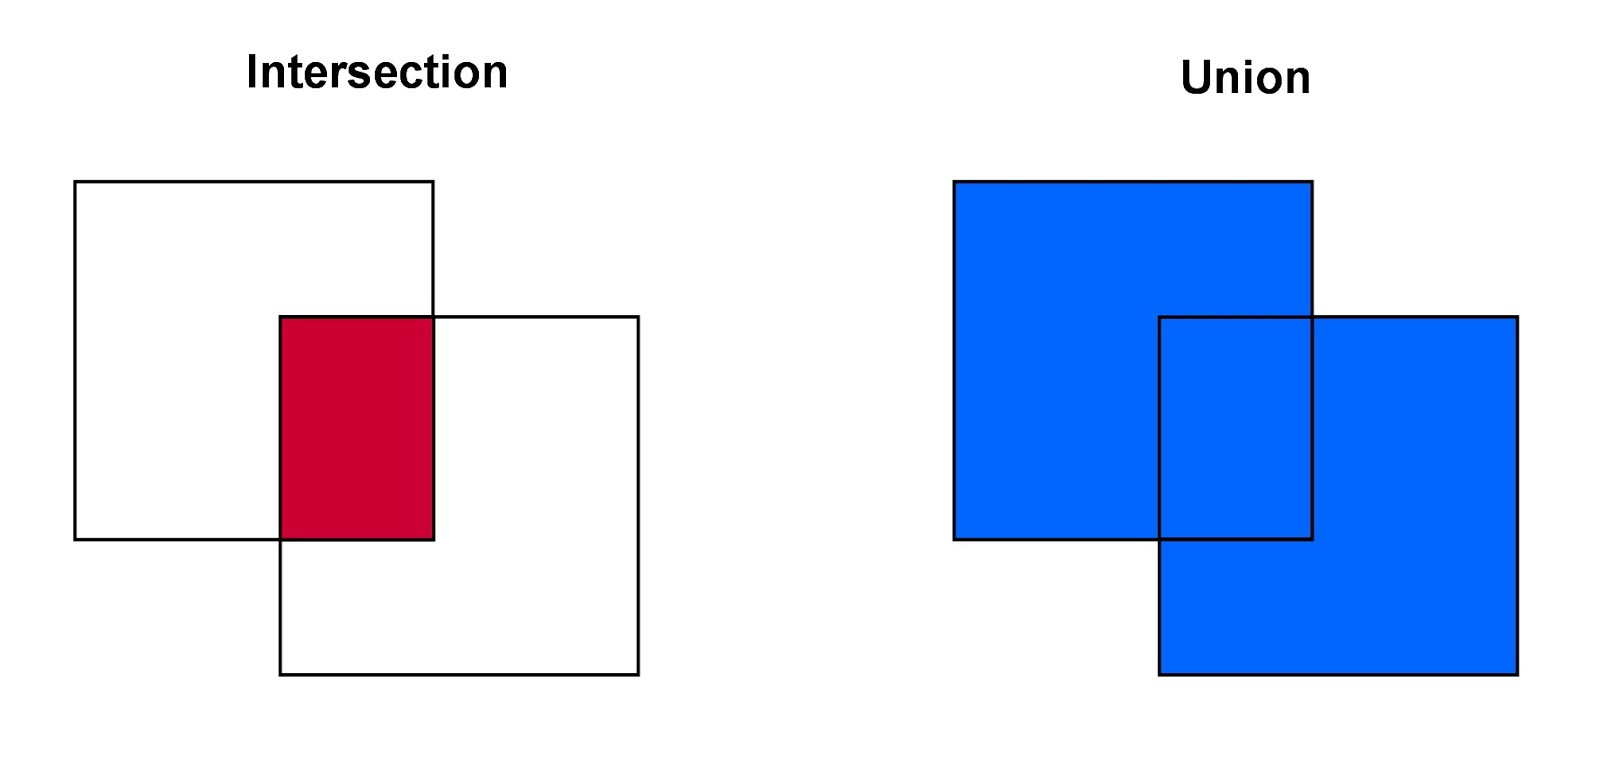
\includegraphics[width=0.5\linewidth]{images/unione-intersezione.jpg}
	\caption{Esempio di intersezione e di unione}
	\label{Esempio di intersezione e di unione}
\end{figure}
\subsubsection{Average Precision}
Un'altra delle metriche utilizzate è l'average precision (AP) e per calcolarla si fa la media delle precisioni di undici diversi valori di recall equamente distribuiti. Questa metrica viene applicata ad una sola categoria di elementi e viene calcolata tramite la seguente formula:
\[
    AP = \frac{1}{11}\sum_{Recall\ped{i}}^{} Precision(Recall\ped{i})
\]
Dove \textit{i}=[0, 0.1, 0.2, …, 1.0] in quanto 0 \textless =recall\textless =1. Inoltre la precisione di uno specifico valore di recall viene calcolata nel seguente modo:
\[
    Precision(Recall\ped{i}) = max\,Precision(Recall\ped{j}) \quad \textrm{and} \quad j>=i
\]
L'AP è un valore che riassume la forma della curva precision/recall per una data categoria.
\subsubsection{Mean Average Precision}
La mean average precision (mAP) è la media delle AP di tutte le categorie calcolata su diverse soglie di IoU:
\[
    mAP\ped{IoU=x\%} = \frac{1}{n}\sum_{i=0}^{n}AP\ped{i}
\]
Dove \textit{i} è il numero totale di categorie sulle quali è stata calcolata la propria AP e \textit{x} rappresenta diverse soglie di IoU.

\subsection{Dataset utilizzato per detection su singole immagini}
I test sono stati eseguiti su un dataset di immagini satellitari in alta risoluzione con circa 3000 pixels di altezza e 4000 di larghezza. Il modello di rete è stato allenato per riconoscere elementi appartenenti a sessanta categorie, le quali, verranno riportate nella tabella 1 insieme ai loro relativi risultati. Il dataset utilizzato è particolarmente impegnativo da analizzare a causa delle ambiguità tra molte delle sue categorie in quanto molte di esse rappresentano lo stesso elemento ma sotto forma di tipologie diverse. Per esempio, gli oggetti appartenenti alle categorie dalla 8 alla 17 sono tutti dei camion, ma di diversa tipologia, tanto che perfino un essere umano, se non esperto in materia, farebbe fatica a distinguerli. La seconda difficoltà viene aggiunta dal fatto che le immagini sono state prese da satelliti i quali orbitano ad un'altezza di migliaia di kilometri dalla superficie terrestre. Data l'enorme distanza, gli oggetti di dimensioni minori come le automobili sono molto difficili da individuare ed ancora più complesso lo è classificarli nella loro corretta categoria. E' per questo motivo che viene applicata la frammentazione visto che risulta fondamentale non perdere risoluzione durante la detection. In seguito, svolge un ruolo fondamentale l'algoritmo di ricostruzione dell'immagine frammentata in quanto permette di ricomporre le bounding boxes di quegli elementi che sono stati suddivisi su più regioni. In seguito viene mostrata una delle immagini presa dal dataset utilizzato per calcolare le metriche.
\begin{figure}[H]
	\centering
	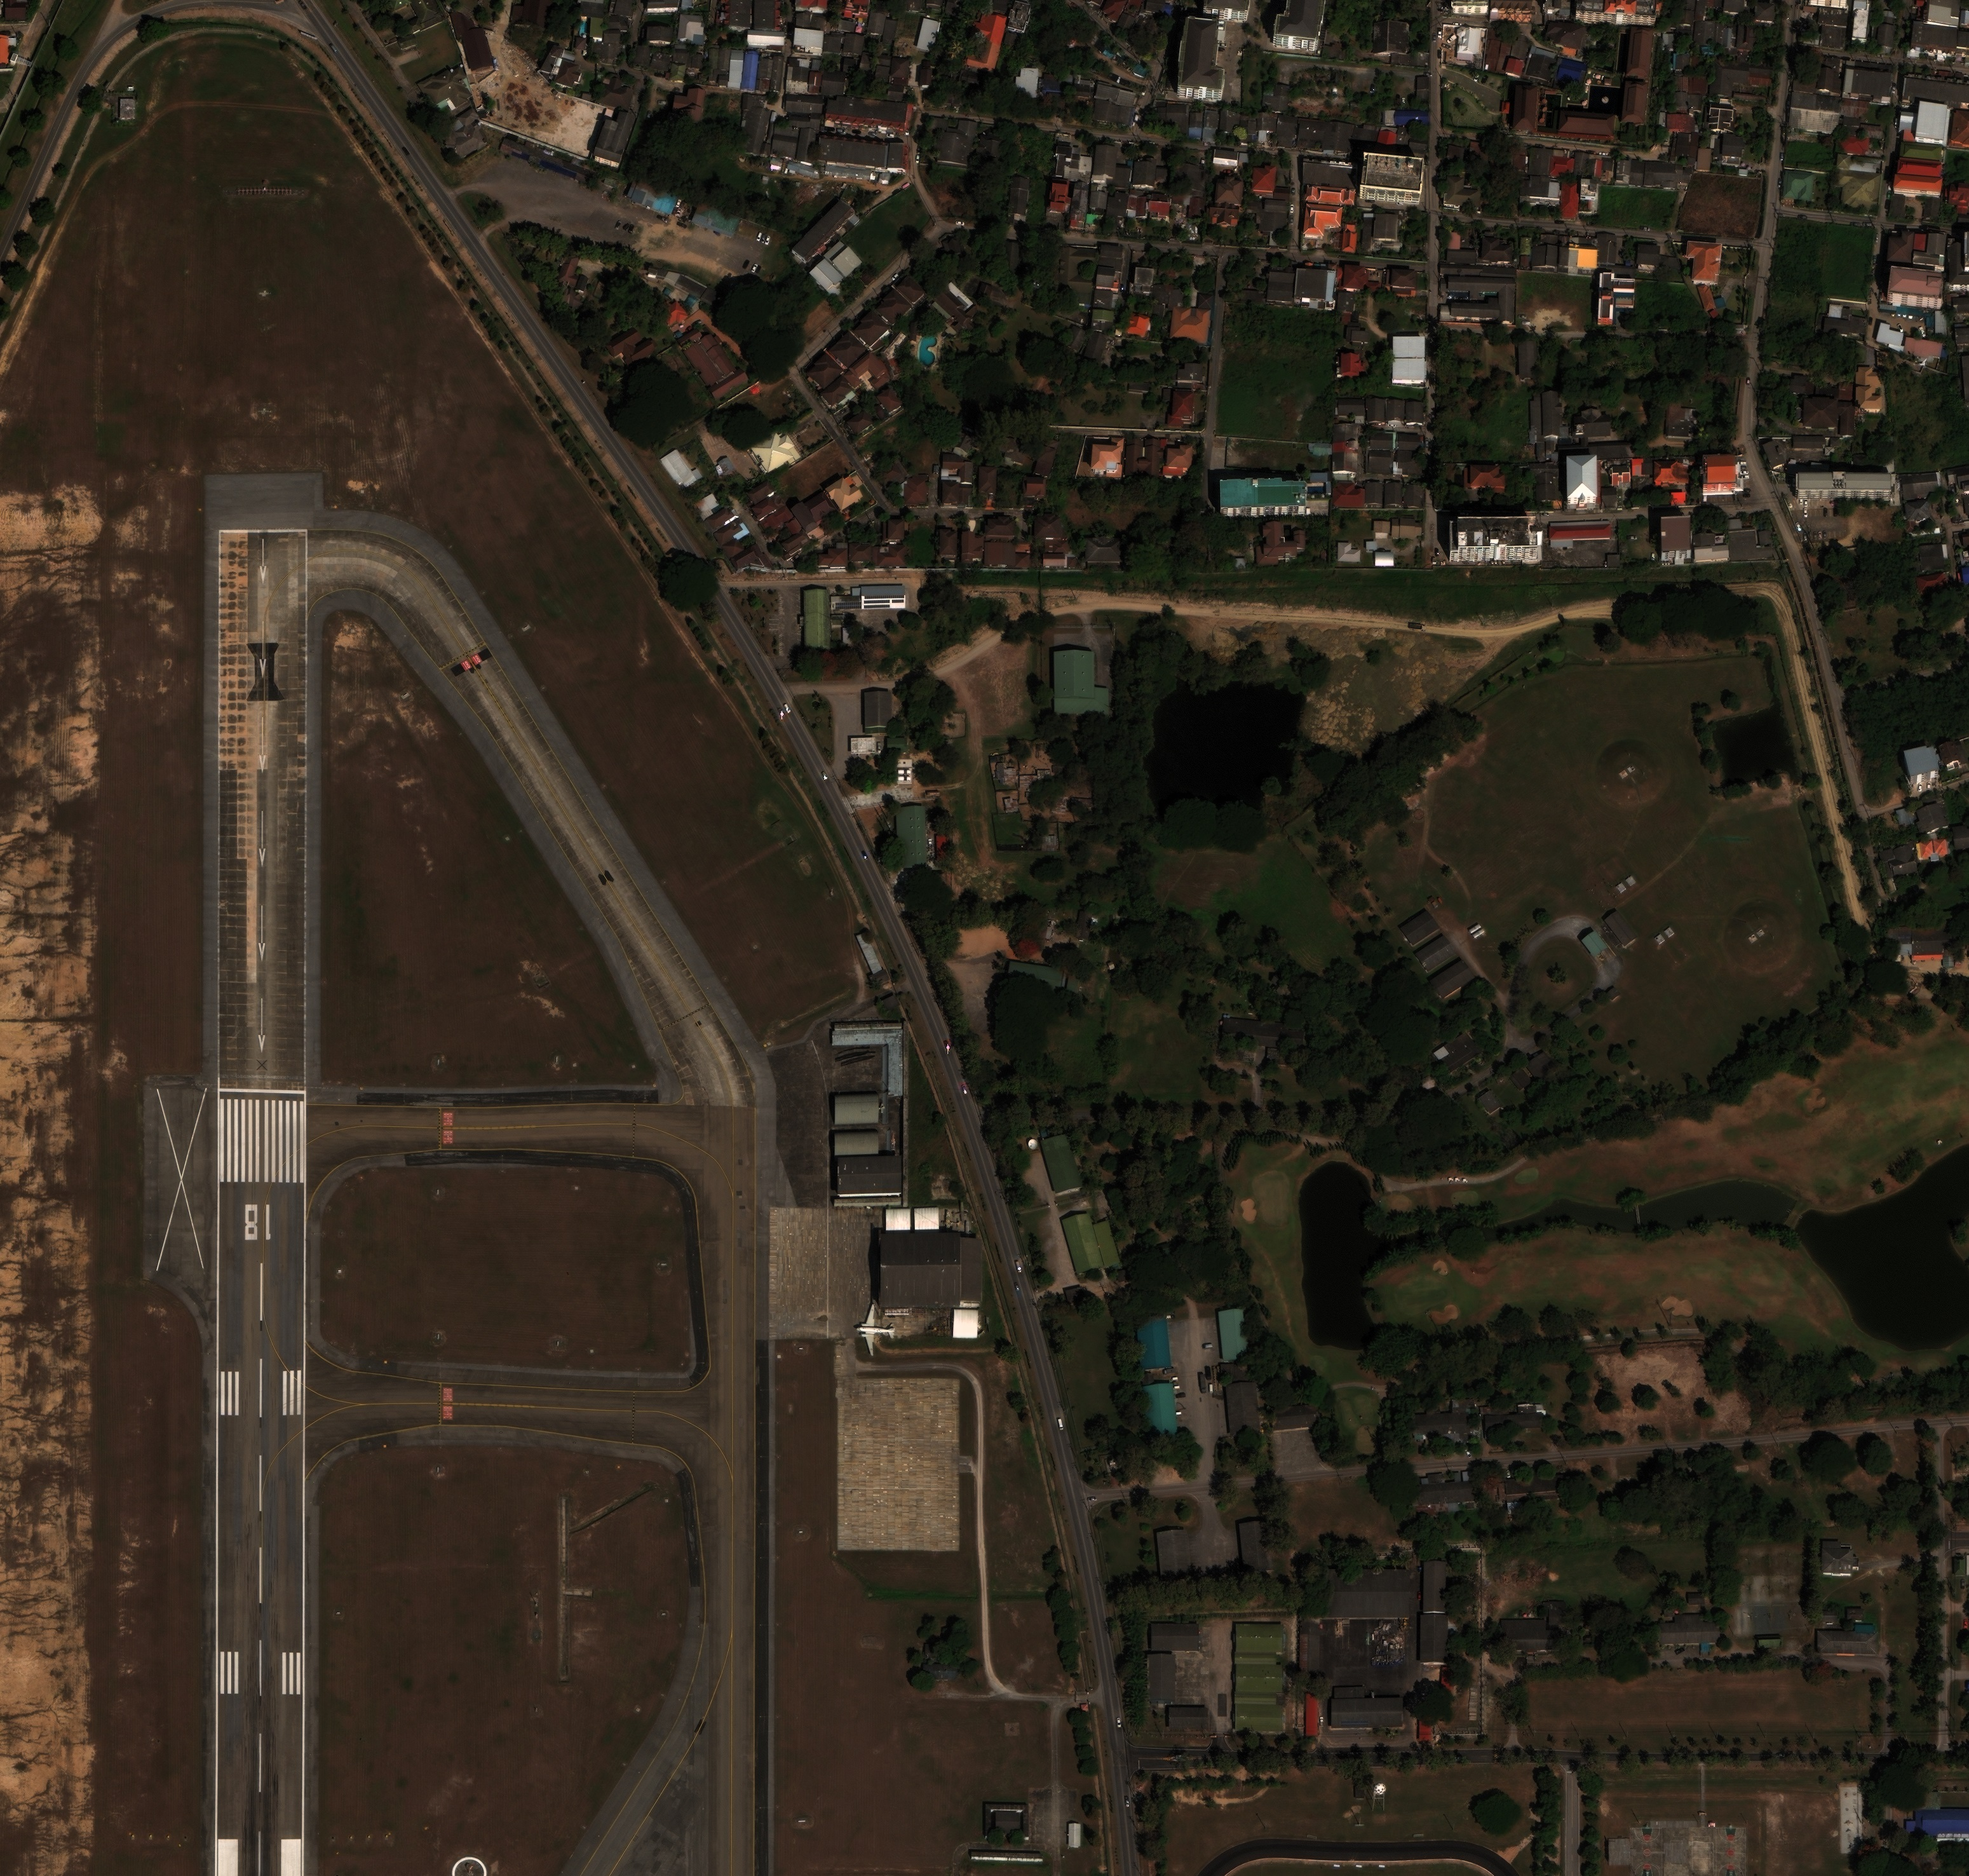
\includegraphics[width=0.7\linewidth]{images/immagine-satellite.jpg}
	\caption{Immagine satellitare appartenente al dataset utilizzato}
	\label{Immagine satellitare appartenente al dataset utilizzato}
\end{figure}

\subsubsection{Impostazione parametri detection}
Il parametro utilizzato per determinare quali labels tenere tra tutte quelle risultanti da una detection è
l' \textbf{affidabilità}.\\
Nella seguente listea vengono elencati i parametri che intervengono in fase di ricostruzione delle labels a seguito della detection:
\begin{itemize}
\item \textbf{Dimensione regioni};
\item \textbf{Dimensione stride};
\item \textbf{Overlap};
\item \textbf{Tolleranza};
\item \textbf{Soglia di matching}.
\end{itemize}
Una spiegazione più dettagliata riguardo ai parametri la si può trovare in sezione \textit{4.1} o nel \textit{Glossario}.
Ogni immagine è stata suddivisa in regioni di dimensioni fisse da 640x640 pixels. A causa della difficoltà nell'individuazione degli elementi, il loro score sarà relativamente basso risultando quindi in una scarsa affidabilità. La \textbf{soglia di affidabilità} per la \textbf{condizione di correlazione} necessaria per effettuare un match è stata perciò impostata a 0. Di conseguenza, due labels di diversa categoria non potranno mai venire unite. Le altre funzioni ridefinibili sono state lasciate con il loro comportamento di default descritto in sezione \textit{4.1}. I restanti parametri sono invece variabili e ne sono state testate diverse combinazioni ai fini di ricercare quelle combinazioni di parametri in grado di fornire i risultati migliori.
\\
La detection è stata effettuata su 100 immagini dove per ciascuna sono state testate 4 soglie diverse di \textbf{affidabilità}=[0.01, 0.1, 0.2, 0.3], 5 valori di \textbf{overlap}=[0, 1, 2, 3, 4], 5 di \textbf{tolleranza}=[0, 1, 2, 4, 4], 4 \textbf{soglie di matching}=[20\%, 40\%, 60\%, 80\%] per un totale di 625 combinazioni di parametri diverse. Le metriche sono state calcolate come media delle metriche per ogni combinazione di parametri e per ogni singola immagine.\\
Per quanto riguarda il test, una bounding box individuata tramite detection è considerata come corretta solo se la sua IoU con la bounding box reale è maggiore di una certa soglia di Iou. Questa soglia è la stessa soglia utilizzata per il calcolo di dell'mAP. Per effettuare i test questa soglia è stata fissata al 50\%.

\subsection{Risultati ottenuti nella detection su singole immagini}
Nella seguente sezione vengono riportati i risultati ottenuti per misurare la qualità della detection e della frammentazione.
\subsubsection{Risultati per categoria}
Nella tabella sottostante vengono riportate tutte le 60 categorie coinvolte nel test insieme al loro AP. I valori mostrati sono quelli relativi alla migliore combinazione di parametri per ogni specifica categoria. La detection è stata effettuata con \textbf{affidabilità} 0.01 in quanto questo è il valore che massimizza i valori di AP e mAP. AP (Original) mostra il valore dell'AP dopo avere effettuato la detection con frammentazione, AP (NMS) è il valore dell'AP dopo aver applicato NMS ed infine AP è il valore dell'AP calcolato dopo aver applicato l'algoritmo di ricostruzione dell'immagine frammentata.

\newpage
\begin{center}
\begin{longtable}{|c|l|c|c|c|}

\hline \multicolumn{1}{|c|}{\textbf{Numero}} &
\multicolumn{1}{c|}{\textbf{Categoria}} & \multicolumn{1}{c|}{\textbf{AP (Original)}} &\multicolumn{1}{c|}{\textbf{AP (NMS)}} &\multicolumn{1}{c|}{\textbf{AP}} \\ \hline\endfirsthead

\hline \multicolumn{1}{|c|}{\textbf{Numero}} &
\multicolumn{1}{c|}{\textbf{Categoria}} &\multicolumn{1}{c|}{\textbf{AP (Original)}} &\multicolumn{1}{c|}{\textbf{AP (NMS)}} &\multicolumn{1}{c|}{\textbf{AP}}\\ \hline \endhead

\hline \multicolumn{5}{|c|}{{------ Continua nella pagina successiva ------}} \\ \hline
\endfoot

\hline

\caption{Lista delle categorie del dataset utilizzato per effettuare i test con relativo AP}
\label{lista categorie} \\

\endlastfoot


1 & Fixed-wing Aircraft & 0.224319 & 0.225709 & 0.234913\\
2 & Small Aircraft & 0.423006 & 0.421561 & 0.487984\\
3 & Cargo Plane & 0.793246 & 0.780495 & 0.809706\\
4 & Helicopter & 0.343750 & 0.343750 & 0.455165\\
5 & Passenger Vehicle & 0.000514 & 0.000561 & 0.000616\\
6 & Small Car & 0.360364 & 0.349376 & 0.354816\\
7 & Bus & 0.320155 & 0.319980 & 0.322155\\
8 & Pickup Truck & 0.004013 & 0.003817 & 0.003832\\
9 & Utility Truck & 0.022319 & 0.022180 & 0.022249\\
10 & Truck & 0.093073 & 0.096008 & 0.097272\\
11 & Cargo Truck & 0.112346 & 0.110611 & 0.113069\\
12 & Truck w/Box & 0.405223 & 0.382302 & 0.389924\\
13 & Truck Tractor & 0.011702 & 0.011205 & 0.011360\\
14 & Trailer & 0.128112 & 0.118257 & 0.121111\\
15 & Truck w/Flatbed & 0.083729 & 0.084326 & 0.086383\\
16 & Truck w/Liquid & 0.028560 & 0.029433 & 0.029457\\
17 & Crane Truck & 0.070424 & 0.070487 & 0.103344\\
18 & Railway Vehicle & 0.00000 & 0.00000 & 0.00000\\
19 & Passenger Car & 0.621967 & 0.634951 & 0.653586\\
20 & Cargo Car & 0.528376 & 0.535936 & 0.537790\\
21 & Flat Car & 0.408165 & 0.436869 & 0.436869\\
22 & Tank Car & 0.000501 & 0.000552 & 0.000563\\
23 & Locomotive & 0.492844 & 0.498693 & 0.500454\\
24 & Maritime Vessel & 0.132787 & 0.122395 & 0.137974\\
25 & Motorboat & 0.304536 & 0.309246 & 0.317420\\
26 & Sailboat & 0.476163 & 0.492080 & 0.501056\\
27 & Tugboat & 0.375028 & 0.379075 & 0.385908\\
28 & Barge & 0.229450 & 0.232367 & 0.237915\\
29 & Fishing Vessel & 0.131085 & 0.134347 & 0.145607\\
30 & Ferry & 0.451626 & 0.445131 & 0.494575\\
31 & Yacht & 0.554554 & 0.561531 & 0.583826\\
32 & Container Ship & 0.562968 & 0.555579 & 0.624139\\
33 & Oil Tanker & 0.562263 & 0.615124 & 0.615124\\
34 & Engineering Vehicle & 0.114510 & 0.114657 & 0.116365\\
35 & Tower Crane & 0.012496 & 0.007083 & 0.007517\\
36 & Container Crane & 0.053083 & 0.050028 & 0.060336\\
37 & Reach Stacker & 0.314528 & 0.317667 & 0.320265\\
38 & Straddle Carrier & 0.573863 & 0.572912 & 0.574765\\
39 & Mobile Crane & 0.131302 & 0.139258 & 0.155806\\
40 & Dump Truck & 0.166618 & 0.169499 & 0.169579\\
41 & Haul Truck & 0.868698 & 0.859369 & 0.889144\\
42 & Scraper/Tractor & 0.028915 & 0.028613 & 0.031487\\
43 & Front Loader/Bulldozer & 0.129784 & 0.138587 & 0.140348\\
44 & Excavator & 0.340663 & 0.335421 & 0.336678\\
45 & Cement Mixer & 0.173915 & 0.182477 & 0.182591\\
46 & Ground Grader & 0.266859 & 0.265571 & 0.265616\\
47 & Hut/Tent & 0.025208 & 0.023967 & 0.026293\\
48 & Shed & 0.009840 & 0.009854 & 0.010107\\
49 & Building & 0.535869 & 0.482216 & 0.490359\\
50 & Aircraft Hangar & 0.019961 & 0.025452 & 0.027149\\
51 & Damaged Building & 0.020142 & 0.021223 & 0.022819\\
52 & Facility & 0.125133 & 0.114053 & 0.139637\\
53 & Construction Site & 0.017198 & 0.016450 & 0.016892\\
54 & Vehicle Lot & 0.087038 & 0.081471 & 0.095994\\
55 & Helipad & 0.020963 & 0.022512 & 0.022866\\
56 & Storage Tank & 0.453776 & 0.452578 & 0.474606\\
57 & Shipping Container Lot & 0.159574 & 0.140996 & 0.149238\\
58 & Shipping Container & 0.101220 & 0.102641 & 0.102708\\
59 & Pylon & 0.657612 & 0.661616 & 0.661769\\
60 & Tower & 0.070426 & 0.071527 & 0.071872\\
\end{longtable}
\end{center}

Osservando i risultati si può subito notare che per ogni categoria si ha che AP$>=$AP(NMS) notando quindi un miglioramento delle metriche a seguito dell'applicazione dell'algoritmo. Per alcune categorie si ha che AP$=$AP(NMS), in questi casi significa che nessuna delle bounding boxes relative a quella categoria è stata coinvolta nella frammentazione. Per alcune categorie può succedere che AP(Original) risulti maggiore sia di AP(NMS) che di AP, questo fenomeno si verifica con più frequenza in presenza di molti oggetti parzialmente sovrapposti tra loro. In questo caso NMS potrebbe causare delle imprecisioni scartando delle bounding boxes che dovrebbero essere in realtà mantenute. Alcune categorie come la numero 5 e la numero 8 presentano un valore di AP particolarmente basso. Si tratta di oggetti che a causa della bassa risoluzione risultano molto piccoli ed ambigui perfino per un occhio umano, per cui, anche il modello spesso commette errori nella loro individuazione e classificazione.
\begin{figure}
\begin{center}
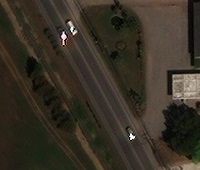
\includegraphics[width=0.4\textwidth, height=0.25\textheight]{images/auto1-satellite.jpg}
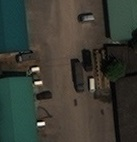
\includegraphics[width=0.4\textwidth, height=0.25\textheight]{images/auto2-satellite.jpg}
\end{center}
\caption{Esempi di oggetti molto difficili da individuare e classificare}
\end{figure}

\clearpage
\subsubsection{Risultati per parametri}
La seguente tabella mostra riporta alcuni dei risultati ottenuti con diverse combinazioni di parametri mostrando i valori di F1 e mAP. mAP(NMS) indica il valore dell'mAp calcolato dopo aver effettuato NMS sull'immagine frammentata mentre mAP è il valore dell'mAP calcolato dopo aver applicato l'algoritmo di ricostruzione dell'immagine frammentata riportandone anche l'aumento in percentuale. Affidabilità è il valore della \textbf{soglia di affidabilità} sopra la quale non scartare una detection.

\begin{table}[h!]
\centering
\begin{tabular}{|c|c|c|c|c|c|c|c|} 
\hline
Affidabilità & Stride & Overlap & Tolleranza & Match(\%) & F1 & mAP(NMS) & mAP\\ [0.5ex] 
\hline
0.01 & 640 & 0 & 0 & 0 & 0 & 0 & 0 (+0.0\%)\\
0.01 & 640 & 0 & 0 & 0 & 0 & 0 & 0 (+0.0\%)\\
0.01 & 640 & 0 & 0 & 0 & 0 & 0 & 0 (+0.0\%)\\
0.01 & 640 & 0 & 0 & 0 & 0 & 0 & 0 (+0.0\%)\\
0.01 & 640 & 0 & 0 & 0 & 0 & 0 & 0 (+0.0\%)\\
0.01 & 640 & 0 & 0 & 0 & 0 & 0 & 0 (+0.0\%)\\
0.1 & 640 & 0 & 0 & 0 & 0 & 0 & 0 (+0.0\%)\\
0.1 & 640 & 0 & 0 & 0 & 0 & 0 & 0 (+0.0\%)\\
0.1 & 640 & 0 & 0 & 0 & 0 & 0 & 0 (+0.0\%)\\
0.1 & 640 & 0 & 0 & 0 & 0 & 0 & 0 (+0.0\%)\\
0.1 & 640 & 0 & 0 & 0 & 0 & 0 & 0 (+0.0\%)\\
0.1 & 640 & 0 & 0 & 0 & 0 & 0 & 0 (+0.0\%)\\
0.2 & 640 & 0 & 0 & 50 & 0 & 0.249199 & 0.250742(+0.0\%)\\
0.2 & 640 & 2 & 4 & 60 & 0 & 0.249199 & 0.253616(+0.0\%)\\
0.2 & 640 & 4 & 4 & 80 & 0 & 0.249199 & 0.252815(+0.0\%)\\
0.2 & 640 & 0 & 0 & 0 & 0 & 0 & 0 (+0.0\%)\\
0.2 & 640 & 0 & 0 & 0 & 0 & 0 & 0 (+0.0\%)\\
0.2 & 640 & 0 & 0 & 0 & 0 & 0 & 0 (+0.0\%)\\
\hline
\end{tabular}
\caption{Risultati generali detection con diversi parametri}
\label{lista risultati}
\end{table}

\subsection{Metriche utilizzate per tracking su video}
L'obiettivo del tracking è quello di identificare tutti gli oggetti in un video e tracciarli nel tempo. Quest'ultimo compito viene svolto assegnando un ID unico a ciascun oggetto assicurandosi che esso rimanga lo stesso per tutta la durata del video. Di conseguenza nel tracking sono due gli aspetti fondamentali di cui tenere conto:
\begin{itemize}
\item Precisione con cui viene determinata la locazione di un oggetto;
\item Correttezza del tracciamento (anche in presenza di occultamento, perdita di qualità, etc...)
\end{itemize}
In seguito vengono descritte le metriche utilizzare per valutare la qualità del tracciamento.

\subsubsection{Mostly Tracked Trajectories}
Mostly Tracked Trajectories (MT), misura la percentuale di elementi, rispetto a quelli totali, che sono stati tracciati correttamente per almeno l'80\% della loro traiettoria. Indica quindi la correttezza del tracciamento, valori più alti sono considerati migliori.
\subsubsection{Mostly Lost Trajectories}
Mostly Lost Trajectories (ML), misura la percentuale di elementi, rispetto a quelli totali, che sono stati tracciati correttamente per non più del 20\% della loro traiettoria. Al contrario di MT, valori più bassi sono considerati migliori.
\subsubsection{ID switches}
ID switches (IDs), viene definito come il numero di volte che un oggetto tracciato cambia il suo ID assegnato. Questo può accadere per esempio nel momento in cui due elementi simili incrociano le loro traiettorie ed i trackers non sono in grado di distinguerli. Anche in questo caso, valori minori esprimono risultati migliori.
\subsubsection{Fragments}
Fragments (FM) conta il numero di volte che una traiettoria viene interrotta durante il tracciamento. Può accadere per esempio a seguito di un occultamento di un elemento, in questo caso un oggetto verrebbe momentaneamente perso e di conseguenza la sua traiettoria risulterebbe frammentata. Valori minori sono considerati migliori. 
\subsubsection{MOTP}
MOTP (Multiple Object Tracking Precision) rappresenta la capacità del sistema di tracking nello stimare con precisione la posizione degli elementi del video attraverso tutti i suoi frames. Viene calcolata nel seguente modo:
\[
MOTP = \frac{\sum_{t}^{}\sum_{i}^{}d\ped{t}\ap{i}}{\sum_{t}^{}c\ped{t}}
\]
Dove \textit{t}=[1,...,n] è l'indice dei frames del video ed \textit{n} è il numero di frames totali, \textit{i}=[1,...,\textit{c\ped{t}}] è l'indice delle associazioni detection-tracker effettuate nel frame \textit{t}, \textit{d\ped{t}\ap{i}} è la distanza tra la posizione reale dell'oggetto \textit{i} e la sua corrispondente posizione stimata nel frame \textit{t}, \textit{c\ped{t}} è il numero di associazioni detection-tracker effettuate nel frame \textit{t}.
\subsubsection{MOTA}
MOTA (Multiple Object Tracking Accuracy) fornisce una misura delle prestazioni del sistema di tracking nel riconoscere gli oggetti presenti nel video e costruire le loro traiettorie. Viene calcolata nel seguente modo:
\[
MOTA = 1-\frac{\sum_{t}^{}(fn\ped{t}+fp\ped{t}+mme\ped{t})}{\sum_{t}^{}g\ped{t}}
\]
Dove \textit{fn\ped{t}} è il numero di falsi negativi, fp\ped{t} è il numero di falsi positivi, mme\ped{t} è il numero di mismatches. Un mismatch avviene quando durante l'associazione detection-tracker un tracker viene associato ad una detection che rappresenta un oggetto diverso da quello associato nel frame precedente. Infine  \textit{g\ped{t}} è il numero di oggetti presenti nel frame \textit{t}.
\subsubsection{IDF1}
IDF1 è una metrica molto simile ad F1 utilizzata come metrica per singole immagini. Questa metrica applicata nell'ambito del tracking fornisce un bilanciamento tra la \textit{precision} media e la \textit{recall} media attraverso la loro media armonica. 
\[
IDF1 = \frac{2IDTP}{2IDTP+IDFP+IDFN}
\]
Dove IDTP, IDFP, IDFN rispettivamente sono la media del numero di detections avvenute correttamente, falsi positivi e falsi negativi calcolati su tutti i frames. 

\subsection{Dataset utilizzato per tracking su video}
Per testare la correttezza del tracciamento sono stati utilizzati alcuni video messi a disposizione dalla sfida VisDrone2019, così come lo è anche lo script utilizzato per calcolare le metriche. I video sono stati girati da alcune telecamere montate su dei droni fatti volare riprendendo diversi scenari che spaziano da aree urbane a zone rurali. I video sono stati girati sotto diverse condizioni meteo, di luminosità a diverse altezze ed angolazioni rendendo quindi particolarmente impegnativi sia il tracking che la detection. Un' ulteriore difficoltà è dovuta al fatto che alcuni frames presentano effetti di sfocatura causata dal movimento. Le dimensioni dei frames variano da video a video così come varia la lunghezza in frames di ogni video. Questa volta sono presenti solamente 5 categorie di oggetti diversi e facilmente distinguibili tra loro:
\begin{itemize}
\item Auto;
\item Bus;
\item Camion;
\item Persona;
\item Furgone.
\end{itemize}
E' da notare la categoria Persona è l'unica categoria che non rappresenta un mezzo di trasporto.

\subsubsection{Impostazione parametri tracking}
Nel tracking entrano in gioco 3 parametri variabili ovvero:
\begin{itemize}
\item \textbf{Soglia di cancellazione};
\item \textbf{Soglia di validazione};
\item \textbf{Soglia di assegnazione}.
\end{itemize}
Una spiegazione più dettagliata riguardo ai parametri la si può trovare in sezione \textit{4.2} o nel \textit{Glossario}.
Per effettuare i test, durante la detection è stata tenuta una \textbf{Soglia di affidabilità} pari a 0.3 e non è stata applicata la frammentazione ai singoli frames in quanto l'operazione sarebbe stata troppo onerosa in termini di tempo mentre usando una Faster-RCNN su ogni frame completo si possono raggiungere qualità di frame-rate accettabili anche per elaborazioni in tempo reale (circa 2 frames al secondo senza utilizzare GPU e con CPU Intel core i5).
Il test è stato effettuato su 7 video, con 3 valori di \textbf{soglia di validazione}=[1, 3, 5], 3 valori di \textbf{soglia di cancellazione}=[1, 5, 10] e due valori di \textbf{soglia di assegnazione}=[0.1, 0.5] per un totale di 18 combinazioni di parametri diverse. Le metriche sono state calcolate su ogni video, su ogni categoria e come media delle metriche per ogni combinazione di parametri.\\
Per quanto riguarda questione dello scambio dell'ID, è da sottolineare che se due oggetti che, incrociando le loro traiettorie, si dovessero ritrovare con un ID diverso, questo evento conterà come 2 scambi di ID invece di 1.

\subsection{Risultati ottenuti nel tracking su video}
Nella seguente sezione vengono riportati i risultati ottenuti per misurare la qualità del sistema di tracking. In quanto l'obiettivo è quello di misurare l'efficacia del tracking e non della detection, quest'ultima non è stata effettuata ma le labels di ogni frames sono state lette da un file di testo contenente le detections esatte, uguali a quelle contenute nel file con il quale vengono confrontati i risultati del tracking ottenuti ai fini di ricavarne le metriche. Successivamente verranno mostrati dei risultati eseguendo le detections con un modello vero e proprio. Le metriche IDF1, Rcll, Prcn, MT, ML, MOTA e MOTP sono espresse sotto forma di percentuali e, ad eccezione di ML, indicano risultati migliori per valori maggiori. Al contrario, le metriche FP, FN, IDs ed FM sono espresse in valore quantitativo ed indicano risultati migliori per valori minori.

\subsubsection{Risultati per categoria}
Nella seguente tabella vengono riportate tutte le cinque categorie insieme ai relativi risultati. Le due metriche Rcll (recall) e Prcn (precision) sono le stesse che sono state utilizzate nella detection su singole immagini ma in questo ambito sono state calcolate come recall e precisione media su ogni frame e su ogni video. I seguenti valori sono stati ottenuti impostando una \textbf{soglia di cancellazione}=1, \textbf{soglia di validazione}=1 e \textbf{soglia di assegnazione}=0.1 in quanto questa combinazione di parametri ha permesso di ottenere risultati migliori rispetto alle altre per quanto riguarda la maggior parte delle metriche.
\begin{table}[h!]
\centering
\begin{tabular}{|c|c|c|c|c|c|c|c|c|c|c|c|} 
\hline
Categoria & IDF1 & Rcll & Prcn & MT & LT & FP & FN & IDs & FM & MOTA & MOTP\\ [0.5ex] 
\hline
Auto & 91.0 & 98.4 & 98.8 & 96.0 & 1.5 & 380 & 505 & 312 & 119 & 96.2 & 93.1 \\
Bus & 93.6 & 95.5 & 99.6 & 100.0 & 0 & 1 & 12 & 7 & 7 & 92.4 & 95.6 \\
Camion & 98.7 & 99.3 & 99.6 & 100.0 & 0 & 6 & 10 & 5 & 2 & 98.5 & 95.0 \\
Persona & 84.7 & 97.8 & 98.7 & 92.4 & 2.2 & 420 & 704 & 462 & 200 & 95.0 & 90.1 \\
Furgone & 93.4 & 98.6 & 99.1 & 95.0 & 0 & 58 & 97 & 32 & 21 & 97.2 & 93.5\\
\hline
\end{tabular}
\caption{Risultati tracking per categoria}
\label{risultati tracking categoria}
\end{table}
In generale è la categoria Persona quella più difficile da tracciare sia per la numerosità delle persone stesse sia per il numero di sovrapposizioni che si verificano tra di esse, lo si può notare dal fatto che le relative metriche sono leggermente più basse rispetto a quelle delle altre categorie.  Le categorie Auto e Persona sono le più frequenti sia nei video sia nel mondo reale perciò è più difficile tracciarle ed aumenta la probabilità che vengano commessi degli errori.

\clearpage
\subsubsection{Risultati per parametri}
La tabella sottostante riporta i risultati ottenuti nel tracking  utilizzando diverse combinazioni parametri SC (\textbf{soglia di cancellazione}), SV (\textbf{soglia di validazione}) ed SA (\textbf{soglia di assegnazione}). Per quanto riguarda il valore dei pesi delle metriche per decidere se validare un assegnazione o meno, è stato dato maggior peso all'IoU ed un peso minore alle metriche che misurano la differenza tra le aree e le dimensioni dei lati.
\begin{table}[h!]
\centering
\begin{tabular}{|c|c|c|c|c|c|c|c|c|c|c|c|c|c|}
\hline
SV & SC & SA & IDF1 & Rcll & Prcn & MT & ML & FP & FN & IDs & FM & MOTA & MOTP\\ [0.5ex] 
\hline
1 & 1 & 0.1 & 88.6 & 98.2 & 98.8 & 94.3 & 1.7 & 865 & 1328 & 818 & 349 & 95.8 & 91.9\\
1 & 1 & 0.5 & 87.7 & 98.1 & 98.8 & 94.3 & 1.9 & 875 & 1359 & 834 & 371 & 95.7 & 91.9\\
1 & 5 & 0.1 & 86.9 & 98.2 & 95.0 & 94.7 & 1.5 & 3684 & 1289 & 889 & 335 & 91.8 & 91.9\\
1 & 5 & 0.5 & 86.3 & 98.2 & 94.8 & 94.7 & 1.7 & 3833 & 1318 & 898 & 368 & 91.6 & 91.9\\
1 & 10 & 0.1 & 84.8 & 98.2 & 90.8 & 95.0 & 1.3 & 7144 & 1265 & 927 & 359 & 87.0 & 91.9\\
1 & 10 & 0.5 & 84.3 & 98.2 & 90.4 & 95.0 & 1.5 & 7463 & 1279 & 956 & 370 & 86.5 & 91.9\\
3 & 1 & 0.1 & 88.5 & 95.9 & 99.1 & 88.7 & 3.2 & 638 & 2948 & 459 & 270 & 94.4 & 92.0\\
3 & 1 & 0.5 & 87.8 & 95.8 & 99.1 & 88.7 & 3.2 & 633 & 3025 & 461 & 275 & 94.3 & 92.0\\
3 & 5 & 0.1 & 87.3 & 96.0 & 96.3 & 89.1 & 3.2 & 2678 & 2903 & 513 & 285 & 91.5 & 92.0\\
3 & 5 & 0.5 & 86.7 & 95.9 & 96.2 & 89.1 & 3.2 & 2734 & 2954 & 522 & 294 & 91.4 & 92.0\\
3 & 10 & 0.1 & 85.7 & 96.0 & 93.0 & 89.1 & 2.7 & 5216 & 2883 & 541 & 298 & 88.0 & 91.9\\
3 & 10 & 0.5 & 85.3 & 95.9 & 92.8 & 89.1 & 2.9 & 5337 & 2921 & 565 & 304 & 87.7 & 92.0\\
5 & 1 & 0.1 & 88.2 & 94.1 & 99.2 & 81.3 & 5.0 & 557 & 4240 & 362 & 233 & 92.8 & 92.1\\
5 & 1 & 0.5 & 87.3 & 94.0 & 99.2 & 80.9 & 5.3 & 553 & 4340 & 366 & 236 & 92.7 & 92.1\\
5 & 5 & 0.1 & 87.1 & 94.2 & 96.7 & 81.7 & 4.8 & 2287 & 4189 & 400 & 254 & 90.4 & 92.0\\
5 & 5 & 0.5 & 86.5 & 94.1 & 96.7 & 81.5 & 4.8 & 2340 & 4239 & 413 & 258 & 90.3 & 92.1\\
5 & 10 & 0.1 & 85.8 & 94.2 & 93.8 & 81.7 & 4.6 & 4437 & 4172 & 423 & 263 & 87.4 & 92.0\\
5 & 10 & 0.5 & 85.3 & 94.1 & 93.6 & 81.7 & 4.6 & 4594 & 4214 & 440 & 265 & 87.1 & 92.1\\
\hline
\end{tabular}
\caption{Risultati tracking per parametri}
\label{risultati tracking per parametri}
\end{table}

Nella tabella si può notare che all'aumentare del valore della \textbf{soglia di validazione} diminuisce il numero di falsi positivi, scambi di ID e di traiettorie frammentate in quanto vengono tracciati meno elementi ma in modo più efficace. Allo stesso tempo, però, le altre metriche tendono a diminuire in quanto elementi di breve comparsa nei video verranno ignorati o solo parzialmente tracciati. All'aumentare della \textbf{soglia di cancellazione} aumenta di molto il numero di falsi positivi al guadagno di una leggera riduzione del numero di falsi negativi ma le altre metriche tendono a rimanere costanti o addirittura peggiorare. Questo è dovuto anche al fatto che in questo caso le detections sono perfette ed il rischio di perdere un elemento tracciato si verifica solo in caso di forte sovrapposizione con altri elementi. Inoltre, le metriche ottenute con \textbf{soglia di accettazione} maggiore sono quasi sempre leggermente inferiori a quelle ottenute con la soglia più bassa, questo perché una soglia alta tende a scartare molte coppie tracker-detection che in realtà sarebbero state corrette, d'altra parte una soglia bassa comporta il rischio di associazioni errate. 

\clearpage
\subsubsection{Risultati per parametri con detection}
La seguente tabella mostra i risultati ottenuti applicando il tracking sul set di video utilizzato in precedenza, questa volta però, gli oggetti sono stati individuati utilizzando un modello per eseguire la detection piuttosto che tramite le loro labels esatte. In questo modo si va a testare il sistema di tracking completo in condizioni reali dove le labels individuate per mezzo della detection non sono esatte ma possono contenere degli errori in grado di influenzare il risultato del tracking stesso. Anche le combinazioni di parametri sono le stesse in modo da poter confrontare i risultati di questa tabella con quelli ottenuti nella tabella precedente.
\begin{table}[h!]
\centering
\begin{tabular}{|c|c|c|c|c|c|c|c|c|c|c|c|c|c|}
\hline
SV & SC & SA & IDF1 & Rcll & Prcn & MT & ML & FP & FN & IDs & FM & MOTA & MOTP\\ [0.5ex] 
\hline
1 & 1 & 0.1 & 50.0 & 68.2 & 81.2 & 69.6 & 16.1 & 5007 & 10076 & 702 & 477 & 50.2 & 84.1\\
1 & 1 & 0.5 & 50.0 & 68.2 & 81.2 & 69.6 & 16.1 & 5009 & 10079 & 702 & 473 & 50.2 & 84.1\\
1 & 5 & 0.1 & 50.2 & 70.0 & 76.5 & 70.5 & 15.6 & 6832 & 9518 & 609 & 431 & 46.5 & 83.6\\
1 & 5 & 0.5 & 49.9 & 70.0 & 76.4 & 70.5 & 15.6 & 6867 & 9512 & 606 & 426 & 46.4 & 83.6\\
1 & 10 & 0.1 & 49.9 & 70.7 & 73.3 & 71.4 & 15.2 & 8155 & 9299 & 578 & 420 & 43.1 & 83.4\\
1 & 10 & 0.5 & 49.7 & 70.7 & 73.2 & 71.4 & 15.2 & 8206 & 9287 & 575 & 418 & 43.0 & 83.4\\
3 & 1 & 0.1 & 50.9 & 66.8 & 83.3 & 69.2 & 16.1 & 4251 & 10535 & 642 & 444 & 51.3 & 84.5\\
3 & 1 & 0.5 & 50.9 & 66.7 & 83.3 & 69.2 & 16.1 & 4249 & 10543 & 641 & 440 & 51.3 & 84.5\\
3 & 5 & 0.1 & 51.0 & 69.1 & 78.5 & 69.6 & 16.1 & 5996 & 9795 & 584 & 412 & 48.3 & 83.8\\
3 & 5 & 0.5 & 50.7 & 69.1 & 78.5 & 70.1 & 16.1 & 6006 & 9794 & 581 & 405 & 48.3 & 83.8\\
3 & 10 & 0.1 & 50.6 & 69.9 & 75.2 & 70.5 & 16.1 & 7324 & 9541 & 561 & 409 & 45.0 & 83.6\\
3 & 10 & 0.5 & 50.4 & 69.9 & 75.2 & 70.5 & 16.1 & 7316 & 9538 & 558 & 406 & 45.1 & 83.6\\
5 & 1 & 0.1 & 51.5 & 65.6 & 84.6 & 68.7 & 16.1 & 3801 & 10893 & 613 & 420 & 51.7 & 84.8\\
5 & 1 & 0.5 & 51.5 & 65.6 & 84.6 & 68.7 & 16.1 & 3797 & 10900 & 614 & 418 & 51.7 & 84.8\\
5 & 5 & 0.1 & 51.5 & 68.4 & 80.1 & 69.2 & 16.1 & 5398 & 10021 & 574 & 400 & 49.5 & 84.0\\
5 & 5 & 0.5 & 51.2 & 68.4 & 80.0 & 69.2 & 16.1 & 5403 & 10021 & 571 & 396 & 49.5 & 84.0\\
5 & 10 & 0.1 & 51.1 & 69.3 & 76.7 & 69.6 & 16.1 & 6674 & 9721 & 552 & 339 & 46.5 & 83.7\\
5 & 10 & 0.5 & 50.9 & 69.3 & 76.7 & 69.6 & 16.1 & 6658 & 9725 & 549 & 397 & 46.6 & 83.7\\
\hline
\end{tabular}
\caption{Risultati tracking per parametri}
\label{risultati tracking per parametri}
\end{table}

Come è facile aspettarsi, quasi tutte le metriche mostrano risultati sensibilmente peggiori rispetto a quelli mostrati nella tabella precedente. In particolare, a causa degli errori introdotti dalla detection risultano esserci molti più falsi negativi e falsi positivi rispetto al tracciamento eseguito con le labels delle detections esatte. A causa del significativo aumento dei falsi negativi è presente una lieve diminuzione del numero di scambi degli ID. Questo comporta un valore MOTA praticamente dimezzato rispetto alla versione precedente mentre la metrica MOTP subisce solo una moderata diminuzione. Per lo stesso motivo anche le metriche Rcll e Prcn presentano valori più bassi riducendo di conseguenza il valore di IDF1.\\
Anche in questo caso i parametri giocano un ruolo fondamentale nel determinare il risultato migliore. Nello specifico, valori alti della \textbf{soglia di validazione} e della \textbf{soglia di cancellazione} aumentano la robustezza del tracciamento a discapito della sua qualità. Infatti i valori di IDs e FM minimi si hanno in corrispondenza dei valori dei parametri SV e SC maggiori. Valori maggiori di SV, filtrando le detections errate, diminuiscono il numero dei falsi positivi mentre valori maggiori di SC, prolungando la durata del tracciamento anche in caso di scomparsa dell'elemento tracciato, riducono il numero di falsi negativi. La metrica IDF1 rimane più o meno stabile per tutte le combinazioni di parametri significando quindi che essa è più influenzata dalla qualità della detection che da quella del tracking. In generale, aumentando le soglie di cancellazione e di validazioni si ha un tracciamento migliore e più resistente agli errori mentre diminuendole si ha un tracking meno preciso ma più completo in quanto verrebbero tracciati un numero maggiore di elementi.